\section{Introducción}
La presente documentación técnica establece los fundamentos teóricos y especificaciones técnicas de los componentes semiconductores y elementos pasivos utilizados en sistemas de control de cargas mediante transistores. El análisis abarca desde los principios fundamentales de la teoría de circuitos hasta las características específicas de los dispositivos semiconductores \citep{malvino2021electronic}.

\subsection{Transistor BJT BD235}
\begin{figure}[H]
	\centering
	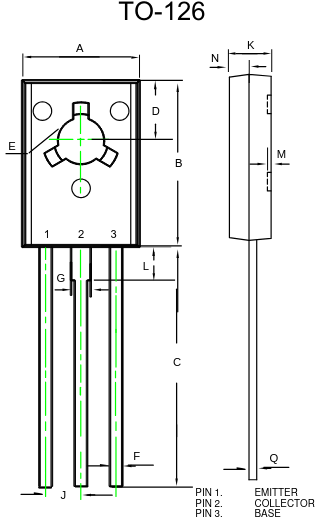
\includegraphics[width=0.3\textwidth]{images/bjt}
	\caption{Transistor BJT BD235 NPN}
	\label{fig:bjt}
\end{figure}
\begin{componentBox}{Especificaciones Técnicas y Configuración \citep{onsemi2021bd235}}
	\begin{itemize}[leftmargin=*,itemsep=1pt,parsep=1pt]
		\item \textbf{Clasificación}: Transistor Bipolar de Unión NPN de Potencia
		\item \textbf{Parámetros Característicos}:
		\begin{itemize}[itemsep=0pt,parsep=0pt]
			\item Tensión colector-emisor máxima (Vceo): \SI{50}{\volt}
			\item Corriente de colector máxima (Ic): \SI{2}{\ampere}
			\item Factor de amplificación de corriente (hFE): 40-250
			\item Configuración física: Encapsulado TO-126
		\end{itemize}
		\item \textbf{Configuración de Terminales}:
		\begin{itemize}[itemsep=0pt,parsep=0pt]
			\item Terminal de Colector (C): Electrodo principal de salida
			\item Terminal de Base (B): Electrodo de control
			\item Terminal de Emisor (E): Electrodo de referencia
		\end{itemize}
	\end{itemize}
\end{componentBox}

\subsection{MOSFET IRLZ44}
\begin{figure}[H]
	\centering
	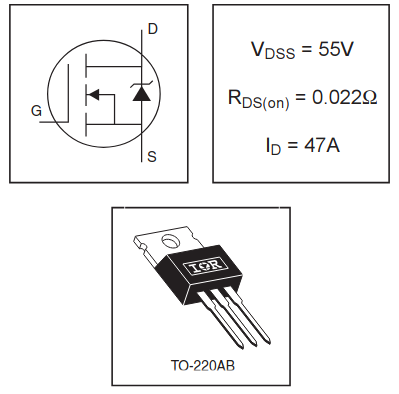
\includegraphics[width=0.3\textwidth]{images/mosfet}
	\caption{Transistor MOSFET IRLZ44N N}
	\label{fig:mosfet}
\end{figure}
\begin{componentBox}{Características Técnicas y Operación \citep{infineon2020irlz44}}
	\begin{itemize}[leftmargin=*,itemsep=1pt,parsep=1pt]
		\item \textbf{Parámetros Operativos}:
		\begin{itemize}[itemsep=0pt,parsep=0pt]
			\item Tensión drenador-fuente máxima (Vds): \SI{55}{\volt}
			\item Corriente de drenador máxima (Id): \SI{47}{\ampere}
			\item Resistencia en conducción (Rds(on)): \SI{0.022}{\ohm}
			\item Tensión umbral de compuerta (Vgs(th)): \SI{1}{\volt}-\SI{2}{\volt}
		\end{itemize}
		\item \textbf{Estructura Terminal}:
		\begin{itemize}[itemsep=0pt,parsep=0pt]
			\item Terminal de Compuerta (G): Control de conducción
			\item Terminal de Drenador (D): Conducción principal
			\item Terminal de Fuente (S): Referencia de potencial
		\end{itemize}
	\end{itemize}
\end{componentBox}

\subsection{Potenciómetro de Precisión \SI{10}{\kilo\ohm}}
\begin{figure}[H]
	\centering
	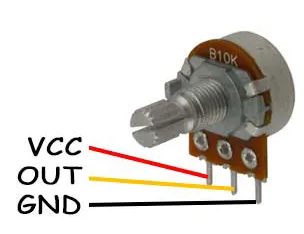
\includegraphics[width=0.3\textwidth]{images/potenciometro}
	\caption{Potenciometro de 10k\ohm}
	\label{fig:potenciometro}
\end{figure}
\begin{componentBox}{Parámetros Técnicos \citep{horowitz2015art}}
	\begin{itemize}[leftmargin=*,itemsep=1pt,parsep=1pt]
		\item \textbf{Especificaciones Fundamentales}:
		\begin{itemize}[itemsep=0pt,parsep=0pt]
			\item Resistencia nominal: \SI{10}{\kilo\ohm}
			\item Configuración mecánica: Sistema rotativo
			\item Característica de variación: Respuesta lineal
		\end{itemize}
		\item \textbf{Disposición de Terminales}:
		\begin{itemize}[itemsep=0pt,parsep=0pt]
			\item Terminal inicial: Punto de referencia
			\item Terminal variable: Cursor de control
			\item Terminal final: Límite resistivo
		\end{itemize}
	\end{itemize}
\end{componentBox}

\subsection{Sistema de Iluminación \SI{12}{\volt}}
\begin{figure}[H]
	\centering
	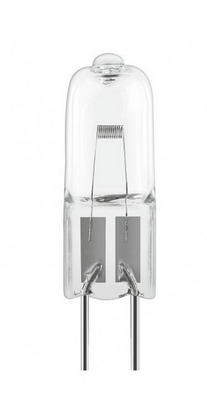
\includegraphics[width=0.3\textwidth]{images/foco}
	\caption{Foco Analógico 12 V a 10 W}
	\label{fig:foco}
\end{figure}
\begin{componentBox}{Parámetros Operativos \citep{boylestad2013electronic}}
	\begin{itemize}[leftmargin=*,itemsep=1pt,parsep=1pt]
		\item \textbf{Especificaciones Eléctricas}:
		\begin{itemize}[itemsep=0pt,parsep=0pt]
			\item Tensión nominal de operación: \SI{12}{\volt}
			\item Potencia nominal: \SI{10}{\watt}
			\item Corriente de operación: \SI{0.83}{\ampere}
		\end{itemize}
	\end{itemize}
\end{componentBox}